\section{Explicación}

\subsection{Definiciones}

\begin{frame}\frametitle{Repositorio}
Se llama \emph{repositorio} (de Git) a una carpeta gestionada por Git.
Se caracterizan por contener una subcarpeta con nombre \cmd{.git}
que contiene toda la información de versiones.

Cuando se usa un repositorio cuya información es accesible desde internet,
como un repositorio en plataformas como \GitHub{} o \GitLab{},
se suele utilizar el nombre repositorio remoto\footnote{
Accesible por internet no implica público.
}.
De forma análoga, se suele utilizar el nombre repositorio local para
un repositorio que se encuentre en un ordenador personal.
La distinción es necesaria porque puede haber varios repositorios para el mismo proyecto,
uno en el ordenador de cada contribuyente y otra versión en GitLab, por ejemplo.
\end{frame}

\begin{frame}\frametitle{\textit{Commit}}
Un \emph{commit} es un conjunto de cambios sobre los archivos de un repositorio,
un punto unívocamente determinado en la historia del proyecto,
que identifica cuál era el contenido de los archivos en ese momento.

\emph{Commit} también es, como verbo, el acto de crear un \textit{commit}.

\vfill
\begin{block}{Te puede interesar}
    \begin{itemize}
        \item Un \textit{commit} se identifica por un código \textit{hash}.
        \item Un \textit{commit} incluye datos como
        el autor, su correo electrónico, la fecha,
        el(los) \textit{commit(s)} padres y
        un mensaje de texto.
        \item El mensaje de texto de un \textit{commit} sirve al resto de colaboradores
        para saber qué cambios aplica ese \textit{commit}.
    \end{itemize}
\end{block}
\end{frame}

\begin{frame}\frametitle{Repositorio Git: Grafo de \textit{commits}}
\hypertarget{fr:graph-example}{}
\small
\begin{figure}[h]
    \centering
    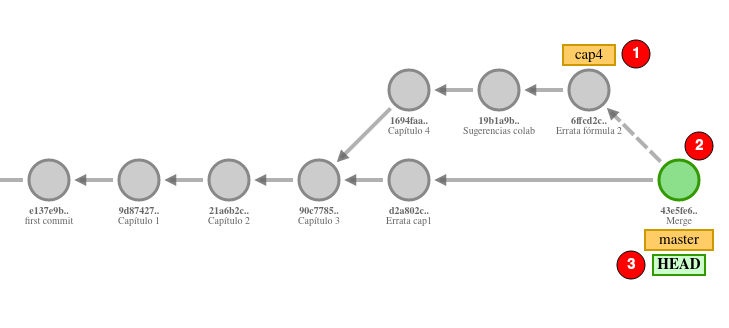
\includegraphics[width=0.85\textwidth]{images/history-example.png}
    \caption{Un ejemplo de historia de un repositorio}
\end{figure}

\begin{enumerate}
    \item Nombre de una rama
    \item Este commit integra los cambios de la rama \cmd{cap4}
    en la rama \cmd{master}
    (que contenía la correción de erratas del capítulo 1 que no estaban en \cmd{cap4}).
    \item \cmd{HEAD} es una referencia al \textit{commit}
    en el que se basa nuestro directorio de trabajo.
\end{enumerate}
\end{frame}

\begin{frame}\frametitle{Ejercicio 2}
\begin{center}
    \Huge
    Aprendemos a manejar la historia con la herramienta

    \href{http://git-school.github.io/visualizing-git/}{Visualizing Git}.
\end{center}
\end{frame}

\begin{frame}\frametitle{\textit{Staging Area}}
En git, para hacer un commit primero tenemos que añadir los archivos a una zona
intermedia que no es el grafo de versiones y se llama \textit{staging area}.
Esto nos permite, por ejemplo,
seleccionar solo los cambios sobre unos archivos para el próximo \textit{commit}.

\vfill
\begin{block}{Un pequeño avance...}
    \begin{itemize}
        \item Los cambios sobre un fichero se registran igual que los ficheros nuevos,
        con el comando \cmd{git add <file>...}.

        \item También se pueden mover/renombrar ficheros con
        \cmd{git mv <current\_file> <new\_file>}
        y borrarlos (ya no se quieren tener en los nuevos \textit{commits}) con
        \cmd{git rm <file>...}.
    \end{itemize}
\end{block}
\end{frame}

\subsection{Qué se puede hacer con un repositorio Git}

\begin{frame}\frametitle{\textit{Diff}}
\begin{figure}[h]
    \centering
    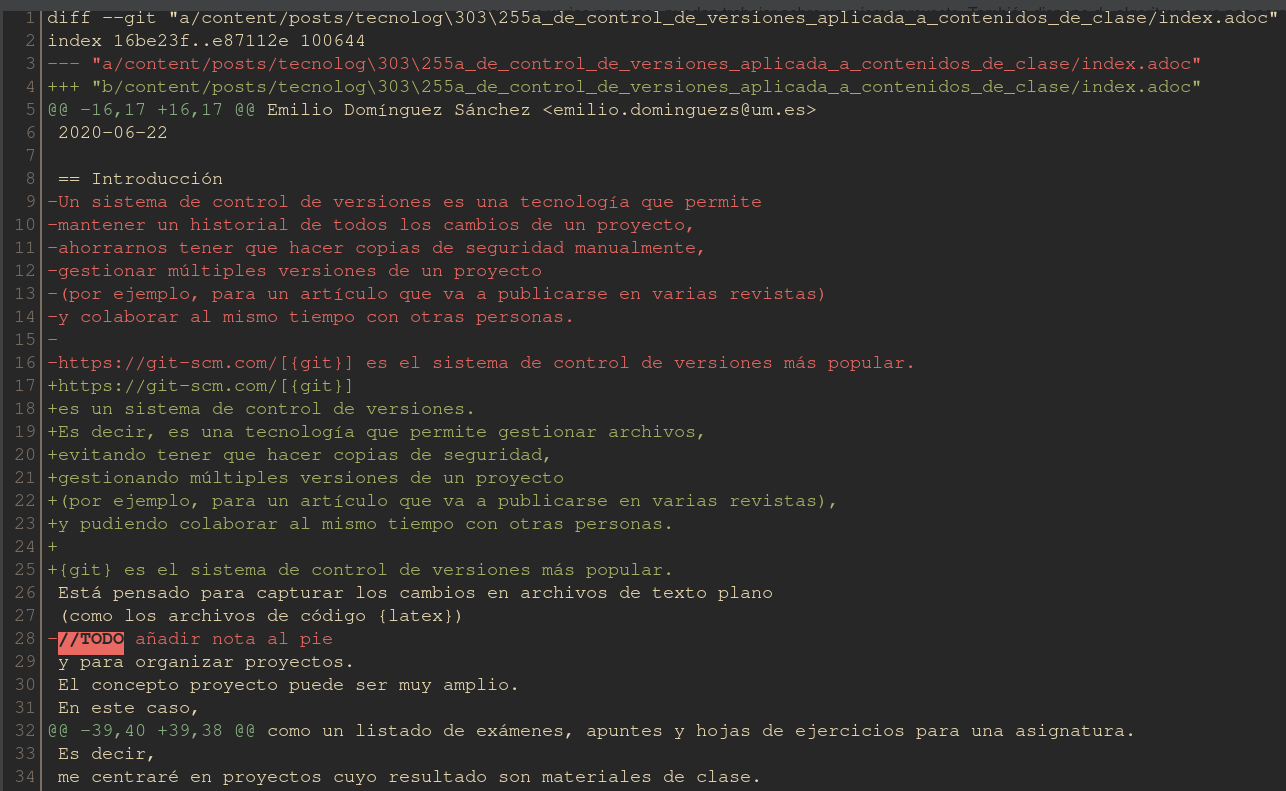
\includegraphics[width=0.85\textwidth]{images/diff-example.png}
    \caption{Salida del comando \cmd{git diff}}
\end{figure}

\href{https://github.com/alberto-ros/apuntes-aec/commit/8b114293d0a19697f0a8db69a6c8005bb6af8911}{\beamerbutton{Un ejemplo en GitHub}}
\end{frame}

\begin{frame}\frametitle{\textit{Merge}}
Una operación \textit{merge} incorpora los cambios
de un commit de otra rama del proyecto
en la rama actual
como si los cambios hechos sobre la otra rama desde el punto en el que divergieron
se repitiesen a partir de este momento.
El resultado de la operación es un nuevo commit sobre la rama actual.

Los algoritmos que utiliza Git internamente son capaces de detectar
cuándo los cambios se pueden mezclar de manera automática.
Por ejemplo, si cada rama del proyecto ha modificado archivos distintos,
entonces conservaremos la versión más nueva posible de cada archivo.
Pero si existen dos versiones modificadas del mismo archivo,
es posible que los cambios puedan incorporarse de forma automática o que no.
Cuando pasa lo segundo, se dice que se ha producido un conflicto,
y los usuarios debemos decidir cómo mezclar ambas versiones
para terminar la operación \textit{merge}.
\end{frame}

\defverbatim[colored]\makeset{
\scriptsize
\begin{minted}{latex}
<<<<<<< HEAD
    c(θ) + \qty\Big(\cos(\frac{3π}{2}-θ), \sin(\frac{3π}{2}-θ)) =
    \qty\Big(\text{using } \cos ρ = \sin(ρ + \frac{π}{2})) = \\
    c(θ) + \qty\Big(\sin(2π-θ), \cos(\frac{π}{2}-θ)) =
    \qty\Big(\text{using } \sin -ρ = -\sin ρ) = \\
    c(θ) + \qty\Big(-\sin θ, \cos(\frac{π}{2}-θ)) =
    \qty\Big(\text{using } -\cos ρ = \cos(\frac{π}{2}-ρ)) = \\
    c(θ) + \qty\Big(-\sin θ, -\cos(θ)) =
    \qty\Big(θ, 1) + \qty\Big(-\sin θ, -\cos θ) = \\
=======
    \begin{split}
        c(θ) + \qty\Big(\cos(\frac{3π}{2}-θ), \sin(\frac{3π}{2}-θ)) =
        & \qty\Big(\text{using } \cos(ρ - \frac{π}{2}) = \ \; \sin ρ) = \\
        c(θ) + \qty\Big(\sin(2π-θ), \cos(\frac{π}{2}-θ)) =
        & \qty\Big(\text{using } \sin\Big(-ρ\Big) \ \,  = -\sin ρ) = \\
        c(θ) + \qty\Big(-\sin θ, \cos(\frac{π}{2}-θ)) =
        & \qty\Big(\text{using } \cos(\frac{π}{2}-ρ) = -\cos ρ) = \\
        c(θ) + \qty\Big(-\sin θ, -\cos(θ)) =
        & \qty\Big(θ, 1) + \qty\Big(-\sin θ, -\cos θ) = \\
    \end{split} \\
>>>>>>> v1
\end{minted}
}

\begin{frame}[fragile]\frametitle{Conflicto}
\makeset
\end{frame}

\begin{frame}\frametitle{
\textit{Pull Requests}(\GitHub) y \textit{Merge Requests}(\GitLab)
}
\begin{figure}[h]
    \centering
    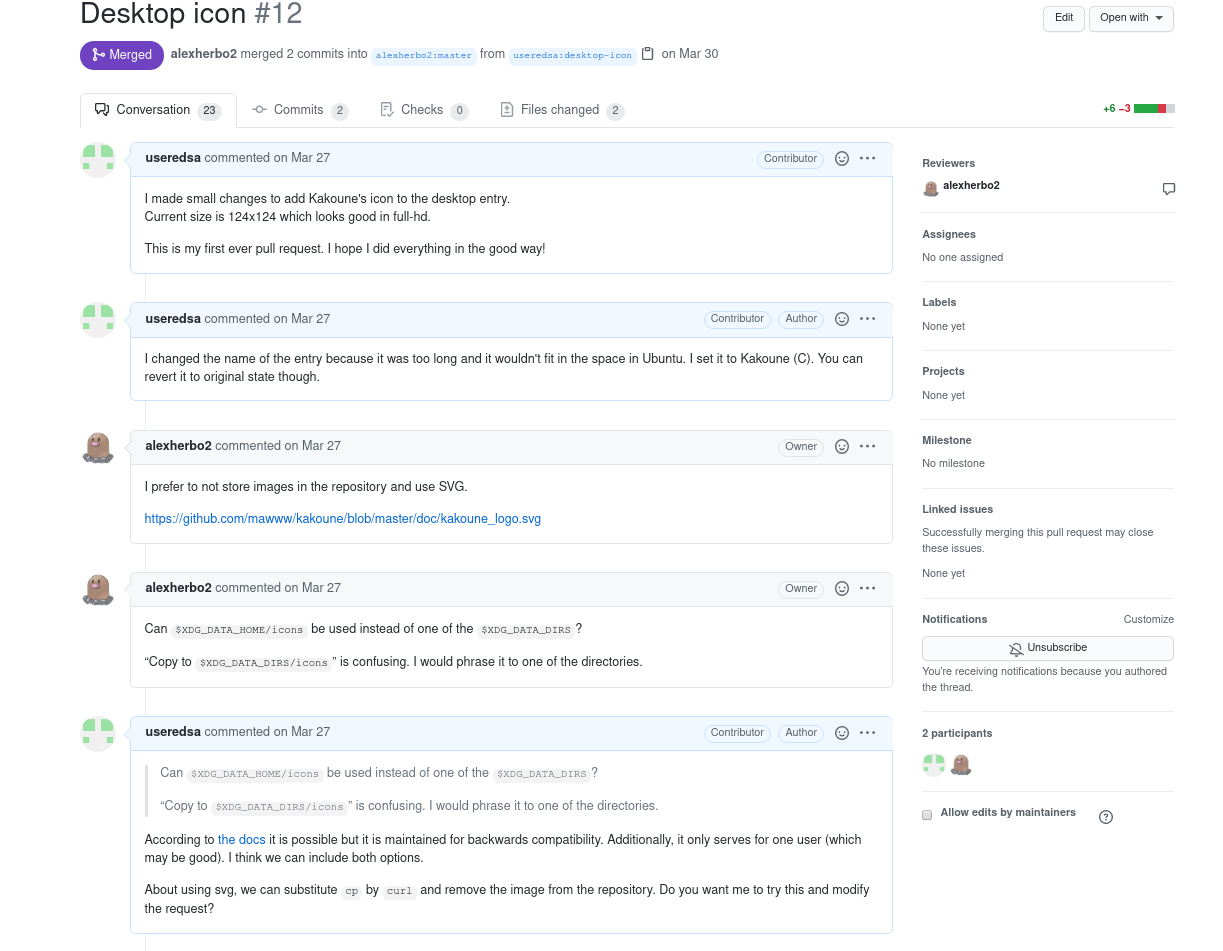
\includegraphics[height=0.7\pageheight]{images/pull-request-example.png}
    \caption{Un \textit{pull request}. El autor puede poner pegas}
\end{figure}

\href{https://github.com/alberto-ros/apuntes-aec/commit/8b114293d0a19697f0a8db69a6c8005bb6af8911}{\beamerbutton{Ver en GitHub}}
\href{https://github.com/useredsa/bspwm.kak/pull/1}{
\beamerbutton{Un ejemplo de correción de erratas}}
\end{frame}

\begin{frame}\frametitle{\textit{Issues}(\GitHub{} o \GitLab{})}
\begin{figure}[h]
    \centering
    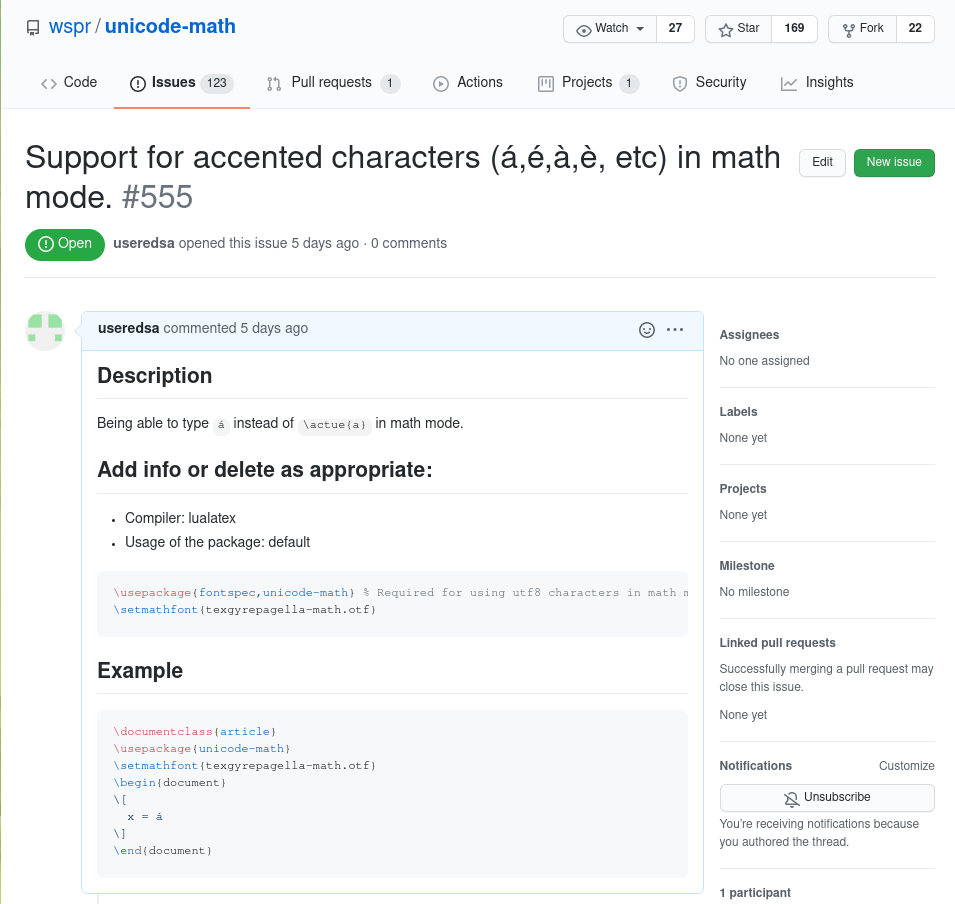
\includegraphics[height=0.7\pageheight]{images/issue-example.png}
    \caption{Un \textit{issue} pidiendo funcionalidad extra en un paquete de LaTex}
\end{figure}

\href{https://github.com/wspr/unicode-math/issues/555}{\beamerbutton{Ver en GitHub}}
\end{frame}

\begin{frame}\frametitle{\textit{Forks}}
\begin{figure}[h]
    \centering
    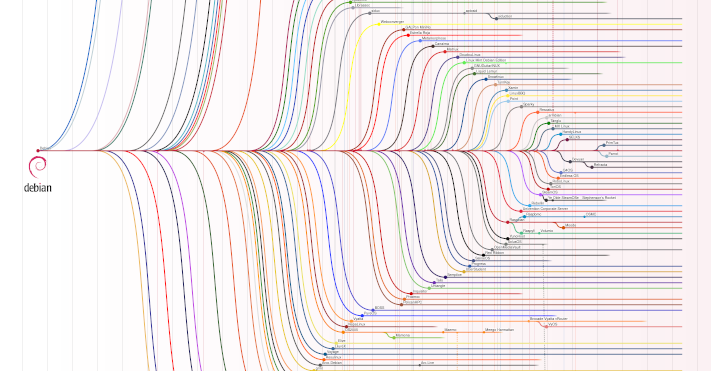
\includegraphics[height=0.65\pageheight]{images/Linux_Distribution_Timeline.png}
    \caption{Origen de las distribuciones de Linux}
\end{figure}

\href{https://upload.wikimedia.org/wikipedia/commons/1/1b/Linux_Distribution_Timeline.svg}{\beamerbutton{Fuente}}
\end{frame}

\subsection{Pre-Comandos}

\begin{frame}\frametitle{Vamos a necesitar...}
Para trabajar con el grafo de \textit{commits} es necesario poder referirse a ellos.
Lo podemos hacer con el \textit{hash} de cada \textit{commit},
pero no es muy práctico.
Vamos a ver otras formas de hacerlo.
\end{frame}

\begin{frame}\frametitle{Tipos de Referencias}
\small
\begin{description}
    \item[Id] El identificador de un \textit{commit} es su código \textit{hash}.
    Es interesante saber que normalmente
    no hace falta escribir el \textit{hash} entero,
    solo hasta el primer caracter que lo indentifique unequívocamente.
    Las salidas de muchos comandos y en muchas herramientas visuales también
    optan por solo escribir un trozo del principio del identificador.
    
    \item[Ramas(\textit{branches})] Una rama es una referencia a un \textit{commit}
    que además cambia automáticamente al siguiente \textit{commit} cada vez que
    estando trabajando sobre esa rama hacemos un nuevo \textit{commit}.
    \hyperlink{fr:graph-example}{\beamerbutton{Grafo}}
    
    \item[\textit{Tags}] Un \textit{tag} es una referencia extra en forma de nombre
    que se puede crear para un \textit{commit} con el comando \cmd{git tag}.
    Por ejemplo, para tener un \textit{commit} llamado \cmd{edicion1}.
    Podría útil si por ejemplo queremos volver a menudo a ese \textit{commit}
    y no está referenciado por ninguna rama ya.

    Mi impresión es que no es algo que utilice gente novata y lo podéis obviar.
\end{description}
\end{frame}

\begin{frame}\frametitle{Tipos de Referencias. Referencias especiales}
\small
Hay algunas referencias especiales que maneja git automáticamente.

\begin{description}
    \item[HEAD] Una referencia que indica sobre qué \textit{commit} estamos trabajando.
    Puede apuntar a una rama,
    en cuyo caso se refiere al \textit{commit} al que apunte esa rama,
    o a un \textit{commit}.
    En el primer caso,
    cuando creemos un nuevo \textit{commit} la rama pasará a apuntar a ese \textit{commit}
    y \textit{HEAD} seguirá apuntado a la rama.
    En el segundo caso,
    \textit{HEAD} pasará a apuntar al nuevo \textit{commit}.

    \item[FETCH\_HEAD] Una referencia al \textit{commit} más avanzado que se ha añadido
    al repositorio con una acción \textit{fetch}.

    \item[Referencias relativas] Hay varios tipos. Lo más importante:

    Una referencia seguida de \cmd{\char`~} indica
    el \textit{commit} padre de esa referencia.
    Una referencia seguida de \cmd{\char`~n}, donde $n$ es un número natural, indica
    el $n$-ésimo padre del \textit{commit} de esa referencia.
\end{description}

\begin{block}{Ejemplo}
    El comando \cmd{git diff HEAD HEAD\char`~1} serviría para ver los cambios
    que ha introducido el \textit{commit} sobre el que estamos.
    El comando \cmd{git reset HEAD\char`~1} serviría para deshacer el último \textit{commit}.
\end{block}
\end{frame}

\subsection{Comandos}

\begin{frame}\frametitle{El mínimo absoluto}
\begin{itemize}
    \item \cmd{git clone <url>}
    \item \colorbox{red}{\cmd{git status}}
    \item \cmd{git add <file>...}
    \item \cmd{git commit -m <mensaje>}
    \item \cmd{git push} y \cmd{git pull}.
\end{itemize}
\end{frame}

\begin{frame}\frametitle{Cosas que nos gustan y acaberemos usando}
\begin{itemize}
    \item \cmd{git diff [<commit\_to>] [<commit\_from>]}
    \item \cmd{git log [--graph]}
\end{itemize}
\end{frame}

\begin{frame}\frametitle{Cosas que usaremos muy de vez en cuando}
\begin{itemize}
    \item \cmd{git config --global user.name "Your Name"} y \\
    \cmd{git config --global user.email "mail@um.es"} \\
    cuando configuremos la herramienta por primera vez en un ordenador.
    \item \cmd{git remote add <remote\_name> <remote\_url>}
\end{itemize}
\end{frame}

\begin{frame}\frametitle{Cuando nos sentimos cómodos es porque podemos usar}
\begin{itemize}
    \item \cmd{git init}
    \item \cmd{git mv}
    \item \cmd{git rm [--staged] <file>}
    \item \cmd{git restore}
\end{itemize}
\begin{itemize}
    \item \cmd{git fetch} y \cmd{git merge}
    \item \cmd{git branch}
    \item \cmd{git checkout (<commit>|<branch>)}
    \item \cmd{git reset}
\end{itemize}
\end{frame}

\begin{frame}\frametitle{Avanzado}
\begin{itemize}
    \item \cmd{git rebase}
    \item \cmd{git revert}
    \item \cmd{git stash}
\end{itemize}
\end{frame}

